%\documentclass{beamer}% Pr�sentation
\documentclass[handout]{beamer}% Handout normal
%\documentclass[hyperref=draft,blackandwhite,slidestop,handout]{beamer}% Stefans options

\usepackage{ngerman}
\usepackage[ansinew]{inputenc}
\usepackage{color}

\usepackage{amsmath}
\usepackage{amsfonts}
\usepackage{amssymb}
\usepackage{tipa}
\usepackage{tipx}
\usepackage{gb4e-}
\usepackage{xyling}

\usetheme{FUBerlin}

% DON'T USE \logo ANYMORE! See changelog of FU texmf tree!
%\logo{
\includegraphics[height=1cm]{fu_dgm_logo}}%

\titlegraphic{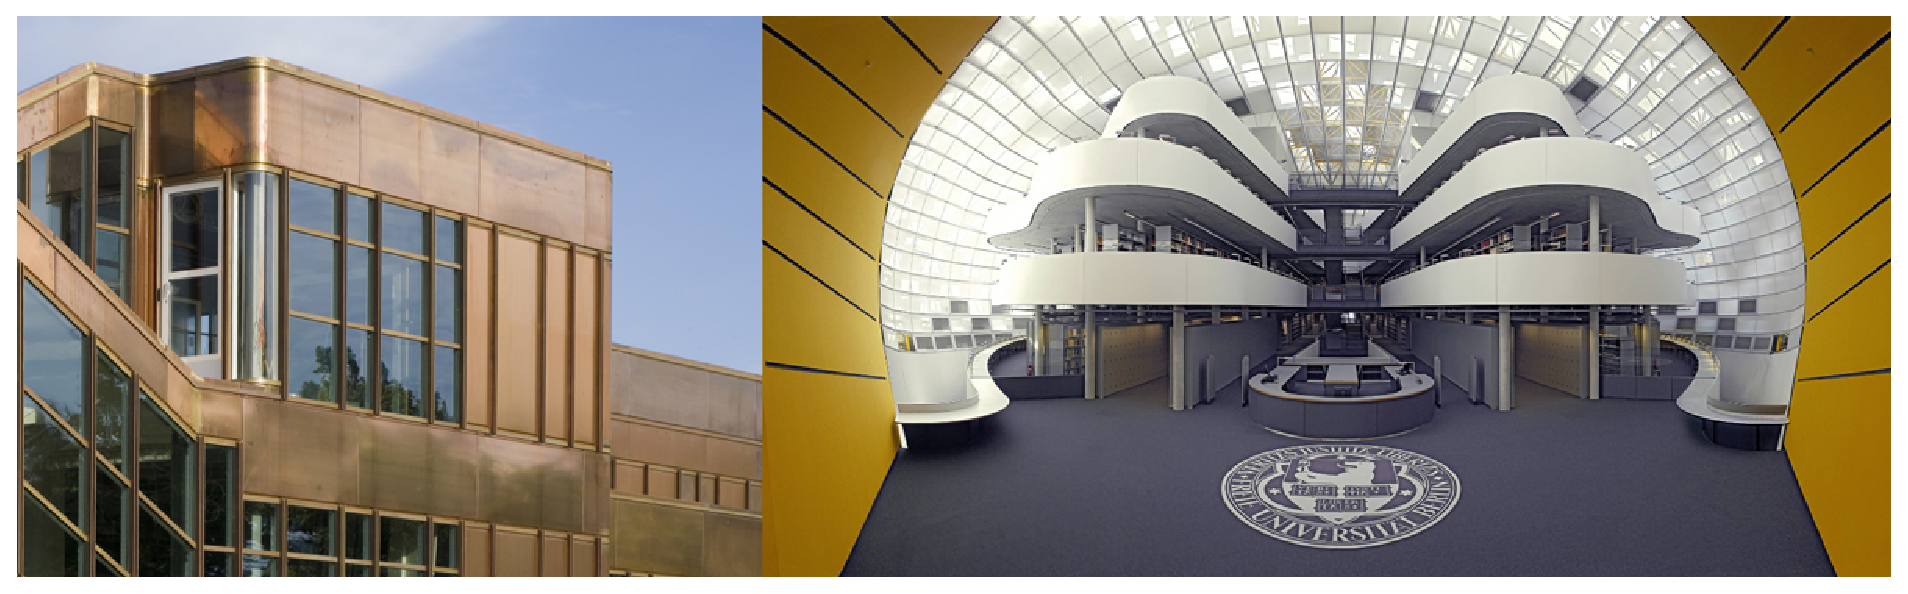
\includegraphics[height=3cm]{fu_dgm}}%

\title[s-title]{l-title}
\subtitle[s-stitle]{l-stitle}
\author[s-author]{l-author}
\institute[s-affiliation]{l-affiliation}
\date{date}


\title[s-title]{l-title}
\author[a-author]{l-author}
\institute[s-inst]{l-inst} 

% use this to change the slide numbering format:
%\renewcommand{\fuberlinpagestring}{\insertpagenumber/\inserttotalpagenumber}

\fuberlinlogon{0.8cm}

\begin{document}

\fuberlintitlepage[12pt]% adjust pt value to displace picture/text block horizontally

\section{s}

\begin{frame}{f}
\begin{itemize}
	\item<1-> \alert{hey}
	\item<2-> .
	\item<3-> .
\end{itemize}	
\end{frame}

\section{s}

\subsection{ss}

\begin{frame}{f}
\begin{itemize}
	\item<1-> \alert{hey}
	\item<2-> .
	\item<3-> .
\end{itemize}	
\end{frame}

\fuberlinpagedec%	do this to decrement the page counter manually
\fuberlinemptyheader
\fuberlinjustbarfootline
\begin{frame}{f}
\begin{itemize}
	\item<1-> \alert{hey}
	\item<2-> .
	\item<3-> .
\end{itemize}	
\end{frame}
\fuberlinnormalfootline
\fuberlinnormalheader

\subsection{ss}

\subsubsection{sss}%

\begin{frame}{f}
\begin{block}{testblock}
testblocktext
\end{block}
\end{frame}

\begin{frame}{f}
\end{frame}

\fuberlinemptyfootline% do this to switch to empty footers
%\fuberlinlastframe% do this to start 'unnumbered' pages. REQUIRED! (Footer won't print if not set!)

%\makeatletter%
%	\setcounter{lastpagemainpart}{\the\c@framenumber}
%\makeatother

\begin{frame}{f}
\begin{itemize}
	\item<1-> \alert{hey}
	\item<2-> .
	\item<3-> .
\end{itemize}	
\end{frame}

\fuberlinlogoff

\begin{frame}{f}
\begin{itemize}
	\item<1-> \alert{hey} logo off
	\item<2-> .
	\item<3-> .
\end{itemize}	
\end{frame}

\begin{frame}{f}
\begin{itemize}
	\item<1-> \alert{hey} logo on again
	\item<2-> .
	\item<3-> .
\end{itemize}	
\end{frame}

\begin{frame}{f}
\begin{itemize}
	\item<1-> \alert{hey} LOGO KLEINER????
	\item<2-> .
	\item<3-> .
\end{itemize}	
\end{frame}

\begin{frame}{f}
\begin{itemize}
	\item<1-> \alert{hey}
	\item<2-> .
	\item<3-> .
\end{itemize}	
\end{frame}

\begin{frame}{f}
\begin{itemize}
	\item<1-> \alert{hey}
	\item<2-> .
	\item<3-> .
\end{itemize}	
\end{frame}

\begin{frame}{f}
\begin{itemize}
	\item<1-> \alert{hey}
	\item<2-> .
	\item<3-> .
\end{itemize}	
\end{frame}

\begin{frame}{f}
\begin{itemize}
	\item<1-> \alert{hey}
	\item<2-> .
	\item<3-> .
\end{itemize}	
\end{frame}

\begin{frame}{f}
\begin{itemize}
	\item<1-> \alert{hey}
	\item<2-> .
	\item<3-> .
\end{itemize}	
\end{frame}

\begin{frame}{f}
\begin{itemize}
	\item<1-> \alert{hey}
	\item<2-> .
	\item<3-> .
\end{itemize}	
\end{frame}

\begin{frame}{f}
\begin{itemize}
	\item<1-> \alert{hey}
	\item<2-> .
	\item<3-> .
\end{itemize}	
\end{frame}

\begin{frame}{f}
\begin{itemize}
	\item<1-> \alert{hey}
	\item<2-> .
	\item<3-> .
\end{itemize}	
\end{frame}

\begin{frame}{f}
\begin{itemize}
	\item<1-> \alert{hey}
	\item<2-> .
	\item<3-> .
\end{itemize}	
\end{frame}

\begin{frame}{f}
\begin{itemize}
	\item<1-> \alert{hey}
	\item<2-> .
	\item<3-> .
\end{itemize}	
\end{frame}

\begin{frame}{f}
\begin{itemize}
	\item<1-> \alert{hey}
	\item<2-> .
	\item<3-> .
\end{itemize}	
\end{frame}

\begin{frame}{f}
\begin{itemize}
	\item<1-> \alert{hey}
	\item<2-> .
	\item<3-> .
\end{itemize}	
\end{frame}

\begin{frame}{f}
\begin{itemize}
	\item<1-> \alert{hey}
	\item<2-> .
	\item<3-> .
\end{itemize}	
\end{frame}

\begin{frame}{f}
\begin{itemize}
	\item<1-> \alert{hey}
	\item<2-> .
	\item<3-> .
\end{itemize}	
\end{frame}
\begin{frame}{f}
\begin{itemize}
	\item<1-> \alert{hey}
	\item<2-> .
	\item<3-> .
\end{itemize}	
\end{frame}

\begin{frame}{f}
\end{frame}

%\fuberlinnormalfootline%		do this to switch back to normal footers

\end{document}